\documentclass[12pt]{article}
\usepackage[utf8]{inputenc}
\usepackage{amssymb}
\usepackage{amsmath}
\usepackage{graphicx}
\graphicspath{{figs/}}
\title{AI1110 assignment1}
\author{Bhargava Ram Rajulapati, CS21BTECH11052}

\begin{document}
  \maketitle
  \section*{Question 6}
  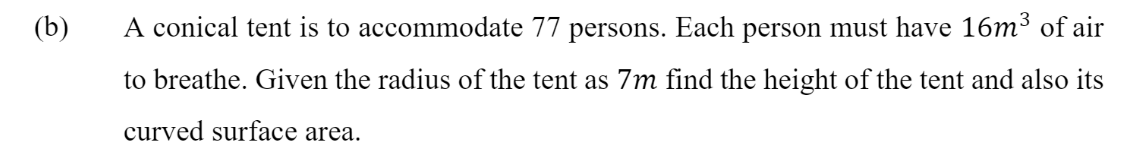
\includegraphics[width=\textwidth]{question.png}\newline
  \section*{Solution:}
  Given a conical tent which can accommodate 77 persons and each         
  person must have $16m^3$ of air to breathe.\newline
  so the volume of conical tent is,\newline
  $  v = 77 \times 16 m^3 $ \newline  \newline
  we know that volume of conical tent is same as a cone having
  radius 'r',height 'h', \newline
  $ v = \frac{\pi r^2 h}{3} $ \newline  \newline
  from the question we are given radius of cone, \newline
  r = 7 m \newline  
  height of cone is \newline
  $ h = \frac{3 v}{\pi r^2} $ \newline
  By substituting values we can get,  \newline
  $ h = 24 m $  \newline  \newline
  Now we know radius and height so we can find lateral height 'l'   
  which is given by,  \newline
  $\hspace*{12pt} l = \sqrt{r^2 + h^2} $  \newline
  $\Rightarrow l = \sqrt{7^2 + 24^2} $ \newline
  $\Rightarrow l = 25 m $ \newline \newline
  we know that lateral/curved surface area 's' of a cone is given
  by, \newline
  $\hspace*{12pt} s = \pi \times r \times l $ \newline
  $\Rightarrow  s = \frac{22}{7} \times 7 \times 25 $ \newline
  $\Rightarrow  s = 550 m^2 $ \newline
  Hence the curved surface area is $ 550 m^2 $. \newline \newline
  The output of the program used to find and verify these numbers
  is: \newline \newline \newline 
  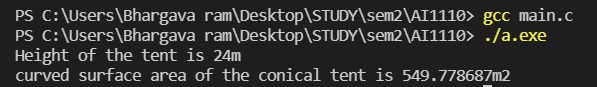
\includegraphics[width=\textwidth]{output.png}\newline   
\end{document}
